



\documentclass[a4paper,12pt,spanish]{article}

\usepackage[utf8]{inputenc}


\usepackage{blindtext}
%\usepackage{microtype}
\usepackage{amsfonts, amsmath, amsthm, amssymb}
%\usepackage{fancyhdr}
%\usepackage{index}
%\usepackage{multicol}    

\usepackage[T1]{fontenc}
\usepackage[utf8]{inputenc}
\usepackage{graphicx}
\usepackage[spanish,es-tabla]{babel}
\usepackage{url}
\usepackage{enumitem}

\usepackage[unicode=true, pdfusetitle,
bookmarks=true,bookmarksnumbered=false,bookmarksopen=false,
breaklinks=true,pdfborder={0 0 1},backref=false,colorlinks=false]
{hyperref}

\usepackage{listings}


\usepackage{siunitx} %para el sistema internacional
\usepackage[export]{adjustbox}
\usepackage{booktabs} 
\usepackage{subcaption}

\usepackage{float}


\newcommand{\address}[1]{
	\par {\raggedright #1
		\vspace{1.4em}
		\noindent\par}
}


\pagenumbering{gobble}
\include{noNumberPage}
\pagenumbering{arabic}
\setcounter{page}{25}

%tutorial de tablas latex: https://manualdelatex.com/tutoriales/tablas

\usepackage{multirow}

% \usepackage[table,xcdraw]{xcolor}


%Inicio del documento (hasta que se cierre con \end{document}
\begin{document}


\title{Cuerda vibrante}

%\author{Adrián Rivero Fernández}
\date{}

\maketitle



\begin{abstract} %resumen
	
En esta práctica usaremos un osciloscopio para estudiar ondas. 
Discriminaremos el primer armónico de una cuerda vibrante, estudiaremos la dependencia de la frecuencia con la longitud de la cuerda y su tensión, y la dependencia de la frecuencia de la cuerda con la densidad del material del que está formada.

	
\end{abstract}

\section{Introducción}

Como en la vibración de una cuerda se producen ondas transversales, y las oscilaciones serán pequeñas, podemos considerar la tensión uniforme a lo largo del hilo, y la fuerza neta en dirección longitudinal nula. Con ello llegamos a que las fuerzas son:
\[F_x = T \cos(\theta + \Delta \theta) - T \cos \theta \approx 0\]
\[F_y = T \sin(\theta + \Delta \theta) - T \sin\theta \approx T\Delta\theta\]

De este modo, para un pequeño trozo de hilo $\Delta x$ de densidad $\mu$, tenemos
\[T\Delta \theta = (\mu \Delta x)a_y
\]
y puesto que $\tan\theta = \frac{\partial y}{\partial x}$,
\[\Delta \theta = \cos^2\theta \frac{\partial^2y}{\partial x^2} \Delta x \approx \frac{\partial^2 y }{\partial x^2}\Delta x\]
y de estas dos podemos deducir que 
\[\frac{\partial^2 y}{\partial x^2}= \frac{\mu}{T}\frac{\partial^2y}{\partial t^2}\]

que se trata de la función de onda, donde la velocidad de propagación es 
\[ v= \sqrt{\frac{T}{\mu}} = \sqrt{\frac{T}{s \rho}} \]

en este último caso hemos relacionado con la densidad volumetrica $\rho$ y la sección $s$. 

Al tratarse de un hilo con los extremos fijos, da lugar a ondas estacionarias. La frecuencia será:
\[f = \frac{nv}{2L} = \frac{1}{2L}\sqrt{\frac{T}{s\rho}}\]


\section{Material y Métodos}


%describir el aparato que hemos montado para este experimento, y el procedimiento que vamos a llevar a cabo para el medimiento, las dificultades, etc.
	
Nuestro dispositivo experimental se compone de un sistema formado por un par de triangulos colocados de forma equidistante a los extremos sobre una regla graduada, de modo que sobre ellos repose un hilo enganchado a un tensador, con un dinamómetro para medir la tensión.
A la altura del hilo tenemos una bombilla de 6V, alimentada por una fuente de alimentación, y en frente una fotocélula con diafragma lineal, de modo que pueda percibir cambios en la luz recibida de la bombilla debido a la oscilación del cable.
Esta fotocélula está conectada a un osciloscopio que nos permitirá visualizarlo.

Disponemos de cables de distinta sección y materiales.

Tendremos que tener precaución con el voltaje para la bombilla, y tener cuidado con no sobrepasar los 30N de tensión para los hilos, ya que no aguantarán y se partirán. Golpearemos el hilo de forma suave, y esperaremos un poco para que la oscilación producida se estabilice.

El experimento se separa en cuatro partes. 

\begin{itemize}
	\item{ Dependencia de la frecuencia con la longitud del hilo: con un mismo cable, iremos variando la distancia entre los triangulos de apoyo }
	\item{ Dependencia de la frecuencia con la tensión: con un mismo cable, y a una misma separación de los apoyos, iremos variando la tensión del hilo y midiendo los cambios en la frecuencia }
	\item{ Dependencia de la frecuencia con la densidad: utilizaremos hilos de diferentes materiales y misma sección }
	\item{ Dependencia de la frecuencia con la sección: utilizaremos hilos del mismo material, misma longitud, y misma tensión, pero diferente sección. }
\end{itemize}



\begin{figure}
	\centering
	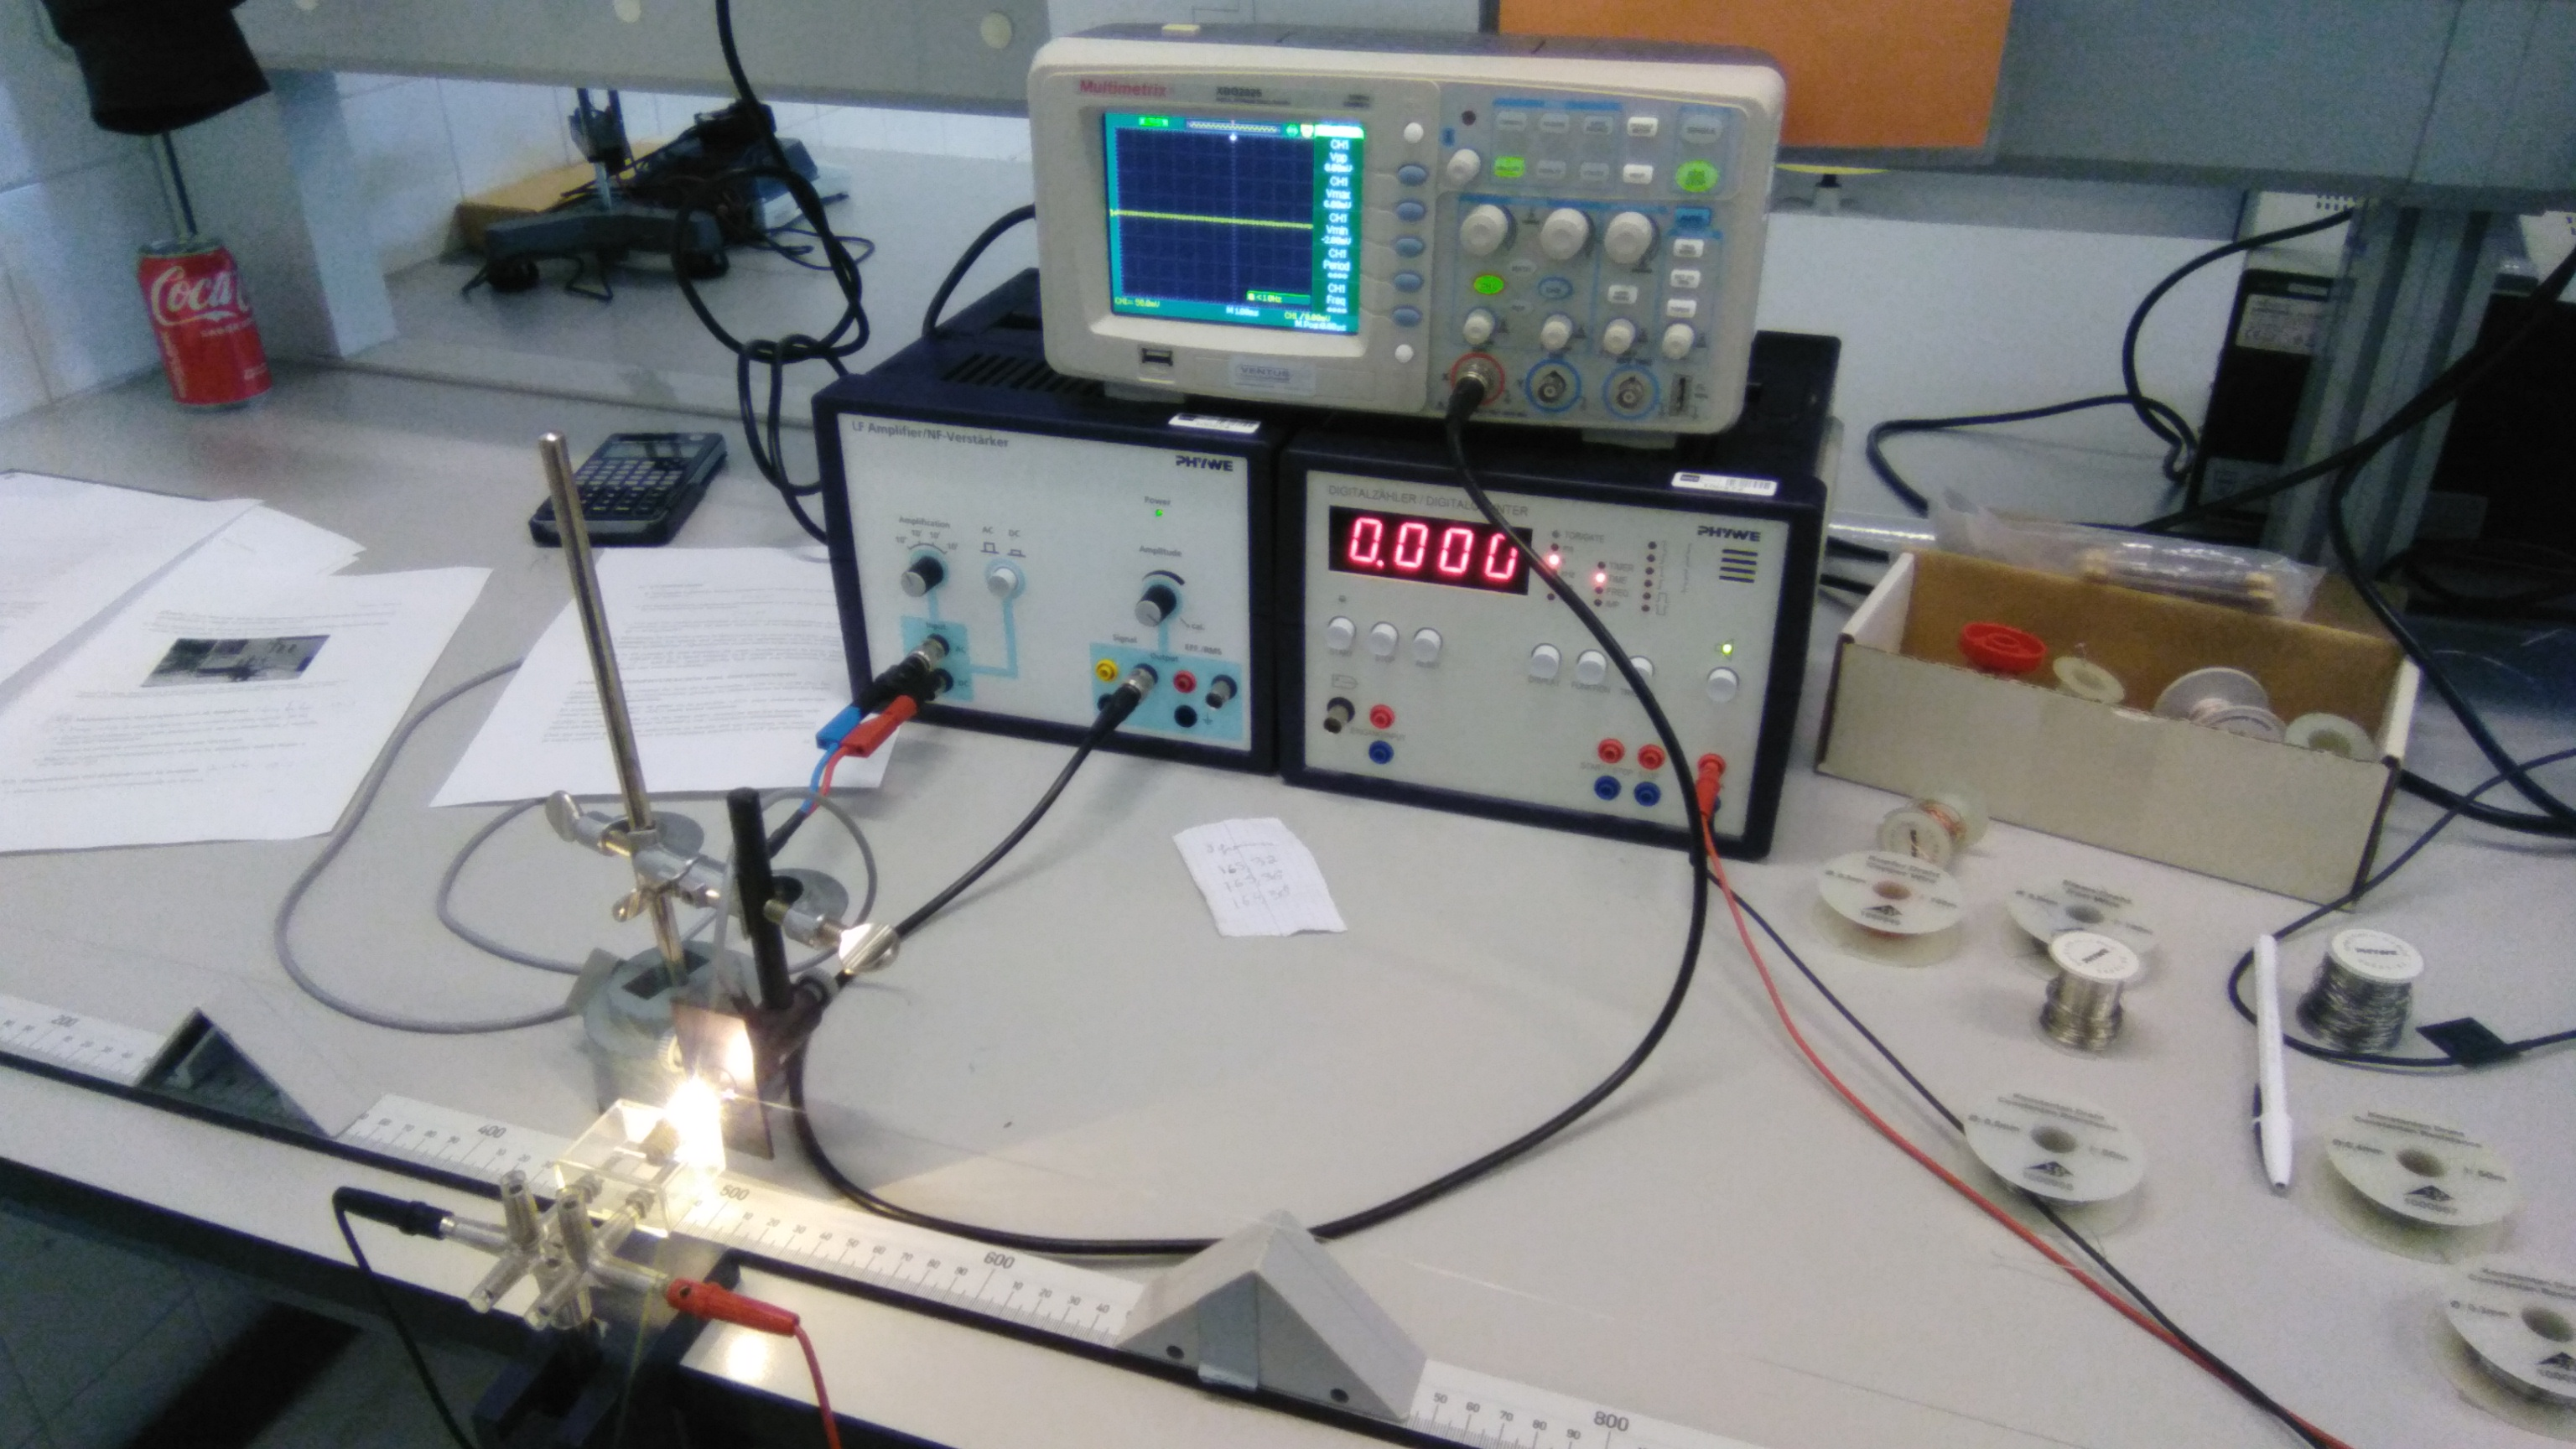
\includegraphics[width=1\linewidth]{../fotos/IMG_20220501_190140}
	\caption{Dispositivo experimental}
	\label{fig:img20220501190140}
\end{figure}



\section{Resultados}

\subsection{ Dependencia con la longitud }
\begin{itemize}
	\item{Hilo: Constatan}
	\item{Sección: 0,3 mm}
	\item{Tensión: 20$\pm 1$N}
\end{itemize}

Frecuencias recogidas en la Tabla 1


\begin{table}[H]
	\begin{minipage}[t]{.48\linewidth}
		\centering
		\begin{tabular}{|l|l|l|}
			\hline
			\textbf{Separación (cm)} & \textbf{20$\pm 0,1$ } \\ \hline 
			Medida 1             & 387,6  $\pm 0,01$   \\ \hline
			Medida 2             & 323,62 $\pm 0,01$    \\ \hline
			Medida 3             & 319,49 $\pm 0,01$    \\ \hline
			Media  (Hz)               & 340 $\pm 20$    \\ \hline\hline
			\textbf{Separación (cm)} & \textbf{30$\pm 0,1$} \\ \hline
			Medida 1             & 229,36 $\pm 0,01$    \\ \hline
			Medida 2            & 228,31 $\pm 0,01$    \\ \hline
			Medida 3             & 229,89 $\pm 0,01$    \\ \hline
			Media  (Hz)               & 229,2 $\pm 0,5$    \\ \hline\hline
			\textbf{Separación (cm)} & \textbf{40$\pm 0,1$} \\ \hline
			Medida 1             & 180,83 $\pm 0,01$    \\ \hline
			Medida 2             & 181,49 $\pm 0,01$   \\ \hline
			Medida 3             & 180,83 $\pm 0,01$    \\ \hline
			Media  (Hz)               & 181,2 $\pm 0,2$     \\ \hline\hline
			\textbf{Separación (cm)} & \textbf{50$\pm 0,1$} \\ \hline
			Medida 1            & 150,83 $\pm 0,01$    \\ \hline
			Medida 2            & 151,06  $\pm 0,01$   \\ \hline
			Medida 3             & 150,83 $\pm 0,01$    \\ \hline
			Media    (Hz)             & 150,83 $\pm 0,08$     \\ \hline
		\end{tabular}
		
	\end{minipage}\hfill
	\mbox{}
	\begin{minipage}[t]{.48\linewidth}% -----------------------tabla 2
		\centering
		\begin{tabular}{|l|l|}
			\hline
			\textbf{Separación (cm)} & \textbf{60$\pm 0,1$} \\ \hline
			Medida 1             & 182,87 $\pm 0,01$    \\ \hline
			Medida 2            & 131,93  $\pm 0,01$   \\ \hline
			Medida 3             & 132,98  $\pm 0,01$   \\ \hline
			Media  (Hz)               & 130  $\pm 20$    \\ \hline\hline
			\textbf{Separación (cm)} & \textbf{70$\pm 0,1$} \\ \hline
			Medida 1            & 111,23  $\pm 0,01$   \\ \hline
			Medida 2            & 111,36  $\pm 0,01$   \\ \hline
			Medida 3            & 112,108 $\pm 0,01$   \\ \hline
			Media (Hz)                & 111,6 $\pm 0,3$    \\ \hline\hline
			\textbf{Separación (cm)} & \textbf{80$\pm 0,1$} \\ \hline
			Medida 1           & 102,04 $\pm 0,01$     \\ \hline
			Medida 2             & 101,11 $\pm 0,01$    \\ \hline
			Medida 3            & 102,67 $\pm 0,01$    \\ \hline
			Media (Hz)               & 101,9  $\pm 0,5$    \\ \hline
		\end{tabular}
		
	\end{minipage}\hfill
	\mbox{}
	\caption{Frecuencia según separación}
\end{table}





\subsection{Dependencia con la tensión}
\begin{itemize}
	\item{Hilo: Constatan}
	\item{Diámetro: 0,3 mm}
	\item{Separación: 50$\pm 0,1$ cm}
\end{itemize}

Frecuencias recogidas en la Tabla 2


\begin{table}[H]
	\begin{minipage}[t]{.48\linewidth}
		\centering
		\begin{tabular}{|l|l|}
			\hline
			\textbf{Tension (N)} & \textbf{10}$\pm 1$ \\ \hline
			Medida 1    & 106,65 $\pm 0,01$     \\ \hline
			Medida 2    & 106,65$\pm 0,01$      \\ \hline
			Medida 3    & 106,65 $\pm 0,01$     \\ \hline
			Media (Hz)   & 106,65  $\pm 0,01$    \\ \hline\hline
			\textbf{Tension (N)} & \textbf{11}$\pm 1$ \\ \hline
			Medida 1    & 111,54 $\pm 0,01$     \\ \hline
			Medida 2    & 111,54 $\pm 0,01$     \\ \hline
			Medida 3    & 108,61 $\pm 0,01$     \\ \hline
			Media (Hz)   & 110  $\pm 1,0$    \\ \hline\hline
		\textbf{Tension (N)} & \textbf{12}$\pm 1$ \\ \hline
			Medida 1    & 121,33 $\pm 0,01$     \\ \hline
			Medida 2    & 117,41 $\pm 0,01$     \\ \hline
			Medida 3    & 116,43 $\pm 0,01$     \\ \hline
			Media (Hz)   & 118,4 $\pm 1,5$       \\ \hline\hline
		\textbf{Tension (N)} & \textbf{13}$\pm 1$ \\ \hline
			Medida 1    & 125,24 $\pm 0,01$     \\ \hline
			Medida 2    & 121,33 $\pm 0,01$     \\ \hline
			Medida 3    & 121,33 $\pm 0,01$     \\ \hline
			Media (Hz)   & 122,6 $\pm 1,3$       \\ \hline\hline
			\textbf{Tension (N)} & \textbf{14}$\pm 1$ \\ \hline
			Medida 1    & 127,20  $\pm 0,01$    \\ \hline
			Medida 2    & 127,20 $\pm 0,01$     \\ \hline
			Medida 3    & 127,20 $\pm 0,01$     \\ \hline
			Media (Hz)   & 127,20  $\pm 0,01$      \\ \hline\hline
		\textbf{Tension (N)} & \textbf{15}$\pm 1$ \\ \hline
			Medida 1    & 133,72 $\pm 0,01$     \\ \hline
			Medida 2    & 132,93 $\pm 0,01$     \\ \hline
			Medida 3    & 132,93 $\pm 0,01$     \\ \hline
			Media (Hz)   & 133,2  $\pm 0,3$      \\ \hline
		\end{tabular}
		
	\end{minipage}\hfill
	\mbox{}
	\begin{minipage}[t]{.48\linewidth}% -----------------------tabla 2
		\centering
		\begin{tabular}{|l|l|}
			\hline
			\textbf{Tension (N)} & \textbf{16}$\pm 1$ \\ \hline
			Medida 1    & 136,01$\pm 0,01$      \\ \hline
			Medida 2    & 136,01 $\pm 0,01$     \\ \hline
			Medida 3    & 135,03 $\pm 0,01$     \\ \hline
			Media (Hz)   & 135,7 $\pm 0,3$       \\ \hline\hline
			\textbf{Tension (N)} & \textbf{17}$\pm 1$ \\ \hline
			Medida 1    & 139,92 $\pm 0,01$     \\ \hline
			Medida 2    & 139,92 $\pm 0,01$     \\ \hline
			Medida 3    & 138,94 $\pm 0,01$     \\ \hline
			Media (Hz)   & 139,6 $\pm 0,3$       \\ \hline\hline
			\textbf{Tension (N)} & \textbf{18}$\pm 1$ \\ \hline
			Medida 1    & 145,79 $\pm 0,01$     \\ \hline
			Medida 2    & 146,77 $\pm 0,01$     \\ \hline
			Medida 3    & 145,79  $\pm 0,01$    \\ \hline
			Media (Hz)   & 146,12  $\pm 0,3$      \\ \hline\hline
		\textbf{Tension (N)} & \textbf{19}$\pm 1$ \\ \hline
			Medida 1    & 147,71 $\pm 0,01$     \\ \hline
			Medida 2    & 147,71 $\pm 0,01$     \\ \hline
			Medida 3    & 147,71  $\pm 0,01$    \\ \hline
			Media (Hz)   & 147,71 $\pm 0,01$       \\ \hline\hline
			\textbf{Tension (N)} & \textbf{20}$\pm 1$ \\ \hline
			Medida 1    & 152,64 $\pm 0,01$     \\ \hline
			Medida 2    & 151,66 $\pm 0,01$     \\ \hline
			Medida 3    & 151,66 $\pm 0,01$     \\ \hline
			Media (Hz)   & 152,0 $\pm 0,3 $       \\ \hline
		\end{tabular}
		
	\end{minipage}\hfill
	\mbox{}
	\caption{Frecuencia según tensión}
\end{table}





 \subsection{Dependencia con la densidad}

\begin{itemize}
	\item{Diámetro: 0,3 mm}
	\item{Separación: 50$\pm 0,1$ cm}
	\item{Tensión: 12$\pm 1$N}
\end{itemize}

Frecuencias recogidas en la Tabla 3



\begin{table}[H]
	\begin{minipage}[t]{.48\linewidth}
		\centering
		\begin{tabular}{|l|l|}
			\hline
			\textbf{Material} & \textbf{Constatan} \\ \hline
			Medida 1          & 121,36  $\pm 0,01$         \\ \hline
			Medida 2          & 117,37$\pm 0,01$            \\ \hline
			Medida 3          & 116,41 $\pm 0,01$          \\ \hline
			Media (Hz)         & 118,4   $\pm 1,5$        \\ \hline\hline
			\textbf{Material} & \textbf{Cobre}     \\ \hline
			Medida 1          & 114,55 $\pm 0,01$           \\ \hline
			Medida 2          & 113,51 $\pm 0,01$           \\ \hline
			Medida 3          & 113,51$\pm 0,01$           \\ \hline
			Media (Hz)         & 113,9  $\pm 0,3$         \\ \hline\hline
			\textbf{Material} & \textbf{Kantal}    \\ \hline
			Medida 1          & 126,26$\pm 0,01$            \\ \hline
			Medida 2          &126,26 $\pm 0,01$           \\ \hline
			Medida 3          & 126,26  $\pm 0,01$          \\ \hline
			Media (Hz)         & 126,26  $\pm 0,01$          \\ \hline
		\end{tabular}
		
	\end{minipage}\hfill
	\mbox{}
	\begin{minipage}[t]{.48\linewidth}% -----------------------tabla 2
		\centering
		\begin{tabular}{|l|l|}
			\hline
			\textbf{Material} & \textbf{Hierro}    \\ \hline
			Medida 1          &120,34 $\pm 0,01$        \\ \hline
			Medida 2          & 119,33$\pm 0,01$            \\ \hline
			Medida 3          & 119,33$\pm 0,01$	            \\ \hline
			Media (Hz)         &119,7 $\pm 0,3$           \\ \hline\hline
			\textbf{Material} & \textbf{Niquel}    \\ \hline
			Medida 1          & 122,25  $\pm 0,01$          \\ \hline
			Medida 2          & 118,34 $\pm 0,01$           \\ \hline
			Medida 3          & 119,33 $\pm 0,01$           \\ \hline
			Media (Hz)         & 120,0  $\pm 1,2$         \\ \hline
		\end{tabular}
		
	\end{minipage}\hfill
	\mbox{}
	\caption{Frecuencia según el material}
\end{table}



\subsection{Dependencia con el diámetro}

\begin{itemize}
	\item{Material: Constatán}
	\item{Separación: 50$\pm 0,1$ cm}
	\item{Tensión: 12$\pm 1$N}
\end{itemize}

Frecuencias recogidas en las Tabla 4


\begin{table}[H]
	\begin{minipage}[t]{.48\linewidth}
		\centering
		\begin{tabular}{|l|l|}
			\hline
			\textbf{Diámetro (mm)} & \textbf{0,2}    \\ \hline
			Medida 1              & 171,23 $\pm 0,01$        \\ \hline
			Medida 2              & 171,23   $\pm 0,01$      \\ \hline
			Medida 3              & 171,23 $\pm 0,01$        \\ \hline
			Media (Hz)             & 171,23  $\pm 0,01$       \\ \hline\hline
			\textbf{Diámetro (mm)} & \textbf{0,3}    \\ \hline
			Medida 2              & 121,36  $\pm 0,01$       \\ \hline
			Medida 3              & 117,37 $\pm 0,01$        \\ \hline
			Medida 4              & 116,41 $\pm 0,01$        \\ \hline
			Media (Hz)             & 118,4  $\pm 1,5$       \\ \hline
		\end{tabular}
		
	\end{minipage}\hfill
	\mbox{}
	\begin{minipage}[t]{.48\linewidth}% -----------------------tabla 2
		\centering
		\begin{tabular}{|l|l|}
			\hline
			\textbf{Diámetro (mm)} & \textbf{0,4}    \\ \hline
			Medida 3              & 86,21 $\pm 0,01$         \\ \hline
			Medida 4              & 86,96 $\pm 0,01$         \\ \hline
			Medida 5              & 86,95  $\pm 0,01$        \\ \hline
			Media (Hz)             & 86,7   $\pm 0,2$       \\ \hline\hline
			\textbf{Diámetro (mm)} & \textbf{0,5}    \\ \hline
			Medida 4              & 70,42 $\pm 0,01$        \\ \hline
			Medida 5              & 70,42 $\pm 0,01$         \\ \hline
			Medida 6              & 70,42 $\pm 0,01$         \\ \hline
			Media (Hz)             & 70,42   $\pm 0,01$       \\ \hline
		\end{tabular}
		
	\end{minipage}\hfill
	\mbox{}
	\caption{Frecuencia según el diámetro}
\end{table}




\section{Discusión}

\begin{itemize}
	\item{En la Tabla 5 y la Figura 2 se representa la frecuencia en función de la distancia. Hemos ajustado mediante regresión lineal}
	
	
	\begin{table}[H]
		\centering
		\begin{tabular}{|c|c|c|}
			\hline
			\textbf{Distancia (m)} & \textbf{Frecuencia (Hz)} & \textbf{$\Delta f$} \\ \hline
			0,2                 & 340                 & 20        \\ \hline
			0,3                 & 229,2               & 0,5        \\ \hline
			0,4                 & 181,2               & 0,2        \\ \hline
			0,5                 & 150,83               & 0,08        \\ \hline
			0,6                 & 130               & 20       \\ \hline
			0,7                 & 111,6               & 0,3       \\ \hline
			0,8                 & 101,9               & 0,5        \\ \hline
		\end{tabular}
		\caption{Frencuencia según distancia}
	\end{table}
	
	
	\begin{figure}[H]
		\centering
		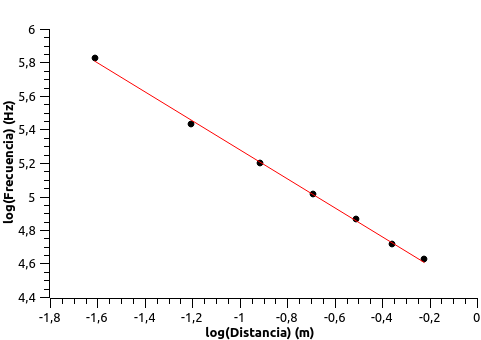
\includegraphics[width=0.8\linewidth]{grafica1}
		\caption{Frecuencia según la distancia}
		\label{fig:grafica1}
	\end{figure}
	
	
	El ajuste nos queda:
	
	\[ y = Ax+B\]
	\[A = -0,86   (\si{Hz/m}) \]
	\[B = 4,42  (\si{Hz})  \]
	
	%B=4.41699580741221
	%A=-0.864564873351967
	%A*x+B
	
	\item{En la Tabla 6 y Figura 3, se representa el logaritmo de la frecuencia frente al logaritmo de tensión, y la recta de ajuste}
	
	
	
	\begin{table}[H]
		\centering
		\begin{tabular}{|l|l|l|l|}
			\hline
			\textbf{Tensión (N)} & \textbf{Frecuencia (Hz)} & \textbf{log(T)}  & \textbf{log(F)}  \\ \hline
			10                   & 106,65 $\pm$0,01              & 1                & 2,03 \\ \hline
			11                   & 110 $\pm$ 1                   & 1,04 & 2,04 \\ \hline
			12                   & 118,4$\pm$  1,5               & 1,08 & 2,07  \\ \hline
			13                   & 122,6 $\pm$ 1,3               & 1,11 & 2,09  \\ \hline
			14                   & 127$\pm$  0,01                & 1,15 & 2,10 \\ \hline
			15                   & 133,2$\pm$  0,3               & 1,18 & 2,12 \\ \hline
			16                   & 135,7 $\pm$ 0,3               & 1,20 & 2,13 \\ \hline
			17                   & 139,6 $\pm$ 0,3               & 1,23 & 2,15 \\ \hline
			18                   & 146,12 $\pm$ 0,3              & 1,26 & 2,16 \\ \hline
			19                   & 147,71 $\pm$ 0,01             & 1,28 & 2,17  \\ \hline
			20                   & 152,0 $\pm$ 0,3               & 1,30 & 2,18 \\ \hline
		\end{tabular}
		\caption{frecuencia según tensión}
	\end{table}
	
	\begin{figure}[H]
		\centering
		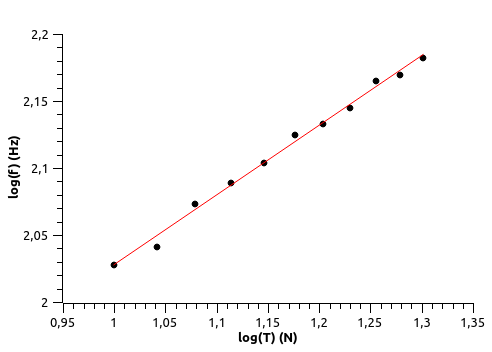
\includegraphics[width=0.8\linewidth]{grafica2}
		\caption{logaritmos de la frecuencia frente a la tensión}
		\label{fig:grafica2}
	\end{figure}
	
	Con el ajuste
	\[ y = Ax+B\]
	\[A = 0.52   (\si{Hz/N}) \]
	\[B = 1.51  (\si{Hz})  \]
	
	%B=1.50770903541901
	%A=0.519877179946638
	
	
	\item{En la Figura 4 hemos representado los logaritmos de frecuencia según los logaritmos de densidad de cada material, especificadas en la Tabla 7.}
	
	
	
	
	\begin{table}[H]
		\centering
		\begin{tabular}{|l|l|l|}
			\hline
			Material  & Densidad (kg/m³)& Frecuencia (Hz) \\ \hline
			constatan & 8966    &  $118 \pm 2 $     \\ \hline
			Cobre     & 8960    &   $113,8\pm0,3$      \\ \hline
			kantal    & 7100    &   $126,26\pm0,01$      \\ \hline
			hierro    & 7874    &   $119,7\pm0,3$      \\ \hline
			niquel    & 8900    &     $120\pm1$    \\ \hline
		\end{tabular}
		\caption{Densidad de los materiales}
	\end{table}
	
	
	
	
	\begin{figure}[H]
		\centering
		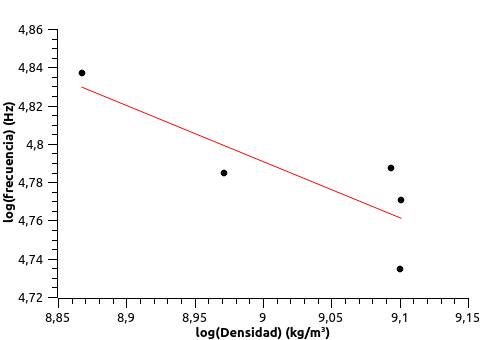
\includegraphics[width=0.8\linewidth]{grafica3}
		\caption{frecuencia según densidad}
		\label{fig:grafica3}
	\end{figure}

	\[ y = Ax+B\]
	\[A = -0.29   (\si{Hz\cdot m^3/kg}) \]
	\[B = 7.43  (\si{Hz})  \]


	
	Vemos que no se ajusta muy bien, posiblemente debido a que algunos materiales presentan diferencias en otras propiedades que afecten a la frecuencia de vibración, a parte de las que hemos estudiado.
	
	\item{En la Figura 5 está representado en escala logarítmica la frecuencia en función del radio del hilo. Podíamos deducir que la frecuencia aumentará a menor radio, ya que implica menor sección, y $ f = \frac{nv}{2L} = \frac{1}{2L}\sqrt{\frac{T}{s\rho}} $}
	
	
	
	\begin{figure}[H]
		\centering
		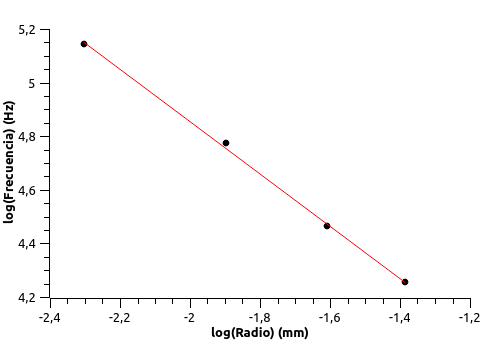
\includegraphics[width=0.8\linewidth]{grafica4}
		\caption{Frecuencia frente al radio}
	\end{figure}
	
	\[ y = Ax+B\]
	\[A = -0,98   (\si{Hz/mm}) \]
	\[B = 2,90  (\si{Hz})  \]
	
	
	
\end{itemize}




\section{Cuestiones}

\textbf{Mediante regresión lineal, encuentre el valor de $\beta$ y su error estándar que ajuste a:}
\[ f = \alpha \cdot L^\beta \]

Del ajuste obtenemos que $\beta= (-0,86 \pm 0,014) \si{Hz/m}$

%-0,864564873351962
%error = 0,014075160421727


	\vspace{\baselineskip}
\textbf{De igual manera, encuentre el exponente $\beta$ y su error para la relación de la frecuencia con la tensión:}
\[ f = \alpha \cdot T^\beta \]

Del ajuste obtenemos $\beta = (0,52 \pm 0,013) \si{Hz/N}$

%0,519877179946607
%0,013194980861424


	\vspace{\baselineskip}
\textbf{¿Por qué las ondas producidas en el cobre parecen distintas de las que aparecen en el níquel, de igual espesor, si su densidad es casi igual ($\rho$ = 8,9 g/cm$^3$)?}
	\vspace{\baselineskip}

Esto es debido a las diferencias en otras propiedades físicas entre estos dos materiales, a parte del espesor o la densidad.


	\vspace{\baselineskip}
\textbf{
	Encontrar la relación entre la frecuencia y la sección del hilo, teniendo presente que los datos del espesor que aparecen en las bobinas se refieren al diámetro. ¿Qué relación existe entre la frecuencia y el radio?
}

La expresión vista en la introducción, 
\[f = \frac{1}{2L}\sqrt{\frac{T}{s\rho}}\]

relaciona la sección $s$ con la frecuencia $f$.

Dado que $s= \pi r^2$, podemos deducir que la relación entre la frecuencia y el radio vendrá dada por:

\[f= \frac{1}{2L}\sqrt{\frac{T}{\pi r^2\rho}}=\frac{1}{2Lr}\sqrt{\frac{T}{\pi \rho}} \]

Al igual que con la sección, la frecuencia se reduce cuanto mayor sea el radio.

	\vspace{\baselineskip}
\textbf{
Si la 6a cuerda de una guitarra da como fundamental la nota "MI" (f = 329,63 Hz) y, a igual tensión, la 5a cuerda proporciona la nota
"LA" (f = 440 Hz), ¿qué relación hay entre sus diámetros, supo-
niéndolas del mismo material?
}
\vspace{\baselineskip}

Aplicamos la anterior expresión, teniendo en cuenta que comparten $L$, $\rho$ y $T$:

\[329,63 = \frac{1}{2Lr_{MI}}\sqrt{\frac{T}{\pi \rho}}\rightarrow 329,63 r_{MI} = \frac{1}{2L}\sqrt{\frac{T}{\pi \rho}}\]
\[ 440 = \frac{1}{2Lr_{LA}}\sqrt{\frac{T}{\pi \rho}}\rightarrow 440 r_{LA} = \frac{1}{2L}\sqrt{\frac{T}{\pi \rho}}
\]

De modo que:
\[ 440 r_{LA} = 329,63 r_{MI}
\]
Y como los diámetros son el doble, la relación será la misma:
\[ \frac{r_{LA}}{r_{MI}}= \frac{329,63}{440} = \frac{d_{LA}}{d_{MI}} \]



	\vspace{\baselineskip}
%%%%%%%%%%%%%%%%%%%%%%%%%%%
\begin{thebibliography}{3}
%%%%%%%%%%%%%%%%%%%%%%%%%%%


\bibitem{UNED2022} (varios) Guiones de prácticas- Técnicas Experimentales II. Grado en Física. Versión 2.1  UNED, 2022 \url{https://2022.cursosvirtuales.uned.es/o/3754218}
\bibitem{UNED2021} (varios) Técnicas Experimentales I. Versión 3.5.  UNED, 2021 \url{https://2021.cursosvirtuales.uned.es/o/42035617}
\bibitem{2021} Densidad de materiales \url{ https://www.stemm.com/index.php/es/densidades-de-materiales }



\end{thebibliography}


\end{document}



